\documentclass[11pt, a4paper]{article}
%\usepackage{proj1}
\usepackage{natbib}
\usepackage{fancyhdr}  
\usepackage{subcaption}
\usepackage{caption}
\usepackage{graphicx}
\linespread{1.25} 
\setlength{\parindent}{0cm}
\graphicspath{{Images/}}
\usepackage{hyperref}
\usepackage{amsmath}
\usepackage{amsfonts}
\usepackage{amssymb}
\usepackage{amsthm}
\usepackage{mathtools}
\usepackage{commath}

%\usepackage[sc,osf]{mathpazo}
\usepackage{subcaption}
\usepackage[a4paper, top=1in, left=1.0in, right=1.0in, bottom=1in, includehead, includefoot]{geometry} %Usually have top as 1in

\usepackage{listings}
\usepackage{color} %red, green, blue, yellow, cyan, magenta, black, white
\definecolor{mygreen}{RGB}{28,172,0} % color values Red, Green, Blue
\definecolor{mylilas}{RGB}{170,55,241}


\hypersetup{colorlinks,linkcolor={black},citecolor={blue},urlcolor={black}}
\usepackage{color}
\urlstyle{same}


\theoremstyle{definition}
\newtheorem{definition}{Definition}[section]

\title{Exact Solutions for the Full Problem \\with Force Control and with Flow Control}
\date{}
\newcommand{\Sta}{\rho}
\newcommand{\Adj}{p}
\newcommand{\Con}{u}

\pagenumbering{gobble}
\begin{document}
\lstset{language=Matlab,%
	%basicstyle=\color{red},
	breaklines=true,%
	morekeywords={matlab2tikz},
	keywordstyle=\color{blue},%
	morekeywords=[2]{1}, keywordstyle=[2]{\color{black}},
	identifierstyle=\color{black},%
	stringstyle=\color{mylilas},
	commentstyle=\color{mygreen},%
	showstringspaces=false,%without this there will be a symbol in the places where there is a space
	numbers=left,%
	numberstyle={\tiny \color{black}},% size of the numbers
	numbersep=9pt, % this defines how far the numbers are from the text
	emph=[1]{for,end,break},emphstyle=[1]\color{blue}, %some words to emphasise
	%emph=[2]{word1,word2}, emphstyle=[2]{style},    
    basicstyle=\footnotesize\ttfamily,
}

\section*{Report on weekly progress; meeting 26/03/2020}
After the 'uniform' perturbation of the control $w$ turned out to be not smooth enough and produced an error at the initial time interval, another perturbation function is trialled:
\begin{align*}
f(t) = \frac{e^{-1/t}}{e^{-1/t} + e^{-1/(1-t)}}.
\end{align*}
When only applying this to the second part of the time interval, it is modified by $\tilde t = t - 0.5$:
\begin{align*}
\tilde f(t) = \frac{e^{-1/(t-0.5)}}{e^{-1/(t-0.5)} + e^{-1/(0.5-t)}}.
\end{align*}
\subsection*{Testing Interpolation on $w$}
Applying $\tilde f$ to $w_{Ex} = \pi e^t(e^T - e^t) \sin(\pi y)(\cos(\pi y)+2))$, the exact solution, means that the second half of the function is perturbed smoothly in time, while the first half remains exact. This is done using $w_{Pert} = w_{Exact}(1 + \tilde f(t))$.\\
The idea is to compare the results of interpolating $w_{Ex}$ and $w_{Pert}$ onto an equispaced grid.
As expected, the first half of the interpolated solution is the same for $w_{Ex}$ and $w_{Pert}$, while there is an increasing difference in the second half.\\
The same can be observed for Dirichlet boundary conditions.
\begin{figure}[h]
	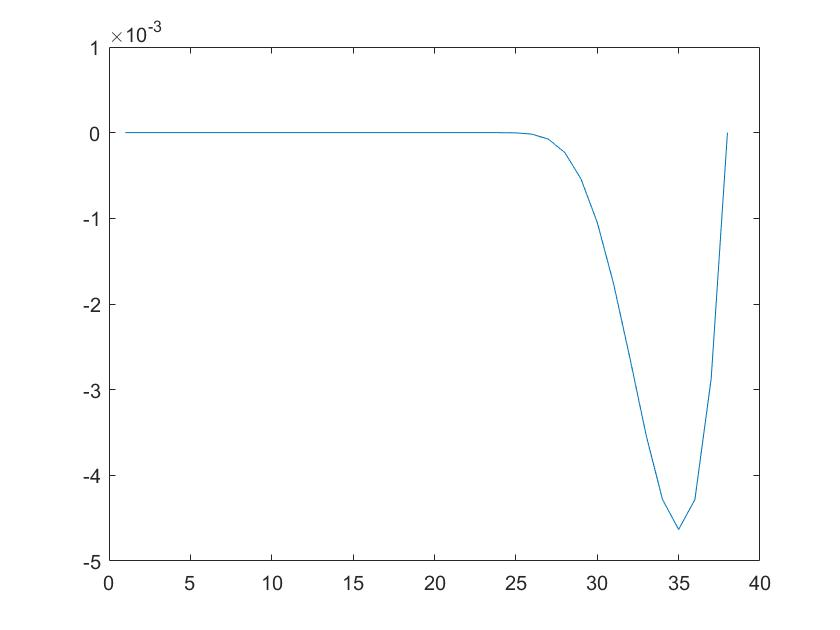
\includegraphics[scale=0.3]{wperthalf.jpg}
	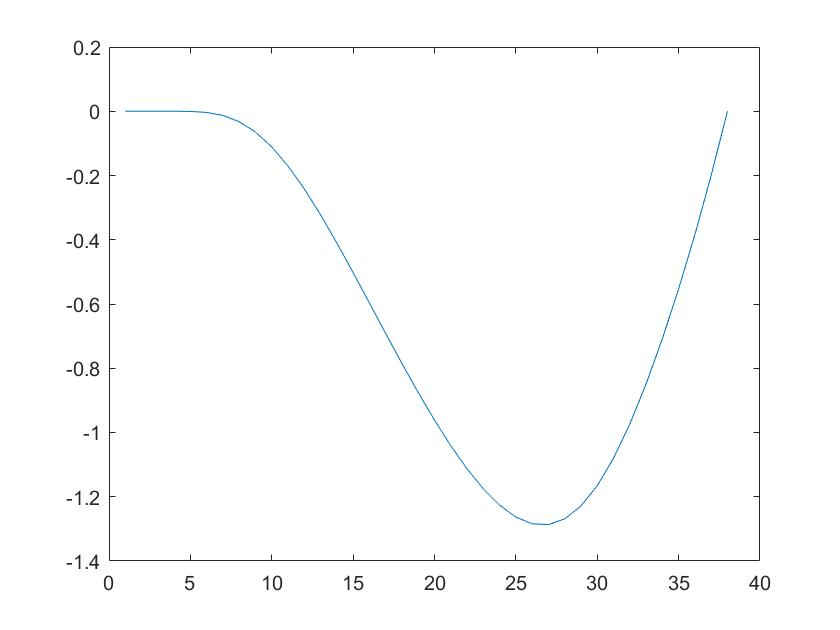
\includegraphics[scale=0.3]{wpertfull.jpg}
	\caption{Perturbing half or whole time interval}
\end{figure}
The most used perturbation in the following is (see Figure 3):
\begin{align*}
w_{Pert} = w_{Ex} (1 + 0.1 f(t)).
\end{align*}
\begin{figure}[h]
	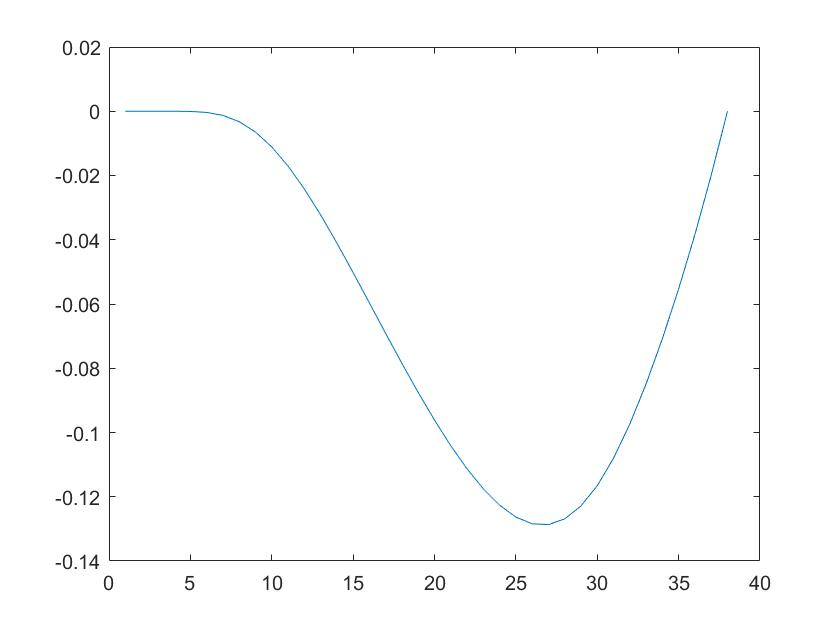
\includegraphics[scale=0.3]{wpertfull01.jpg}
	\caption{Perturbing the whole time interval by $0.1f(t)$.}
\end{figure}
\subsection*{'Kalise' algorithm}
All of the tests are with $\beta = 10^{-1}$, $n = 74$, $N=72$, tolerances for ODE solver are $10^{-12}$ and mostly $\lambda = 0.01$.
\subsubsection*{Neumann Flow Control, shifted by 2 (for positive $\rho$)}
First tried the perturbation of half of the interval by $O(1)$. This converged in $5442$ Iterations, to a consistency in $w$ of $10^{-5}$. The exact errors are $w_{Err}= 9.0243 \times 10^{-5}$, $p_{Err} = 1.0578 \times 10^{-6}$ and $\rho_{Err} = 1.7971 \times 10^{-7}$.\\
Perturbing the whole time interval by $0.1 f(t)$ converges as well, however $p_{Err} = 5.8644 \times 10^-5$. Perturbing by $0.5 f(t)$ does not converge, but only diverges at a consistency of $w_{Cons} = 1.6325 \times 10^{-5}$.
Generally, the error becomes quite erratic at the end ++++ Insert Figure.
\subsubsection*{Dirichlet Flow Control}
 Doing the same thing with the Dirichlet case doesn't work as smoothly. When perturbing half the time interval by $O(1)$, it diverges at a consistency of $w_{Cons} = 2.9520 \times 10^{-5}$. The perturbation $0.1f(t)$ diverges at a consistency of $w_{Cons} = 3.4261 \times 10^{-4}$, for $\lambda = 0.01$ and $\lambda = 0.001$. 



\subsection*{Multiple Shooting Algorithm}
Generally, the configurations are as above, only $\lambda = 0.1$ as a standard and the ODE tolerances are a bit higher $10^{-9}$ or similar.
\subsubsection*{Neumann Flow Control (plus 2)}
All the perturbations tried with the Kalise algorithm do not converge. The code converges up to a point, then diverges. This is mostly of $O(10^{-1}/ 10^{-2})$. 
Tried a perturbation $0.01f(t)$, which also diverges after a while. $\rho$ diverges at Iteration 128 and has error $0.00055580$, $p_{err} = 0.0044...$ and consistency starts diverging a bit earlier at Iteration 105 at $0.00121746$.
The error is very erratic, it looks very unstable, see Figure 4 (and in comparison Figure 3 for initial error).
\begin{figure}[h]
	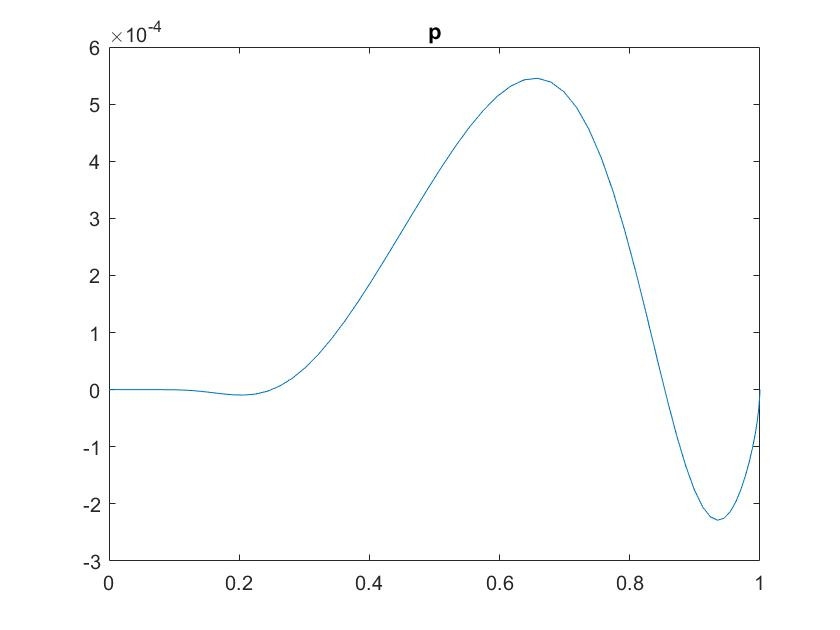
\includegraphics[scale=0.3]{Neumpinit.jpg}
	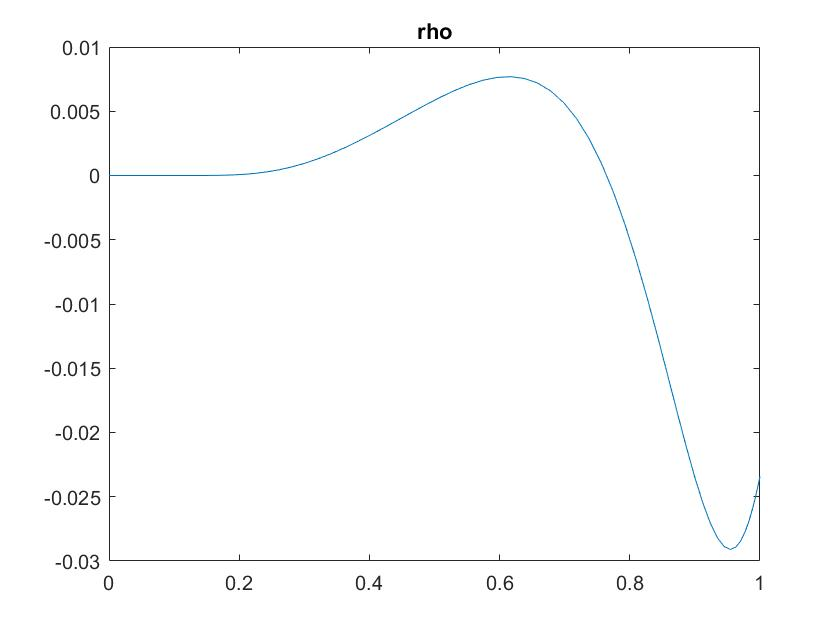
\includegraphics[scale=0.3]{Neumrhoinit.jpg}
	\caption{Initial error in $p$ and $\rho$.}
\end{figure} 
\begin{figure}[h]
	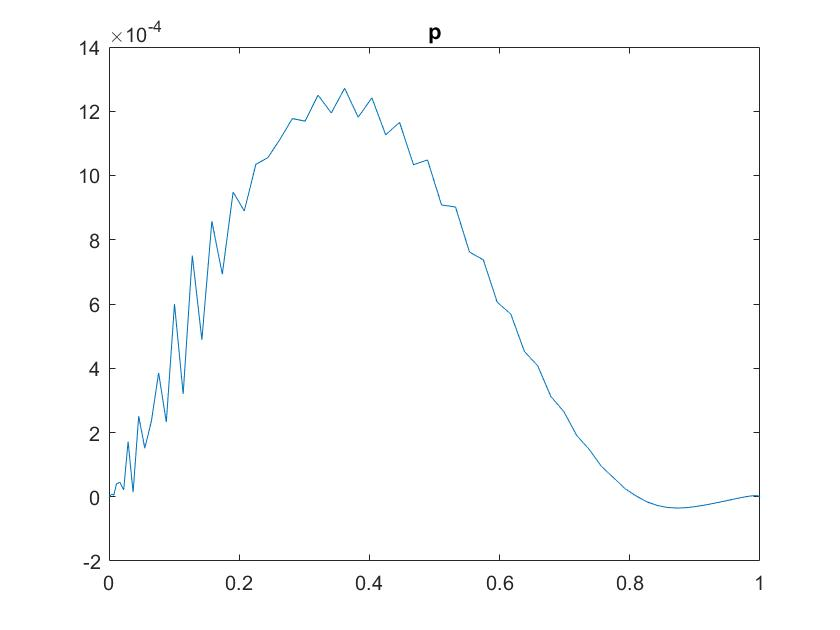
\includegraphics[scale=0.3]{Neump.jpg}
	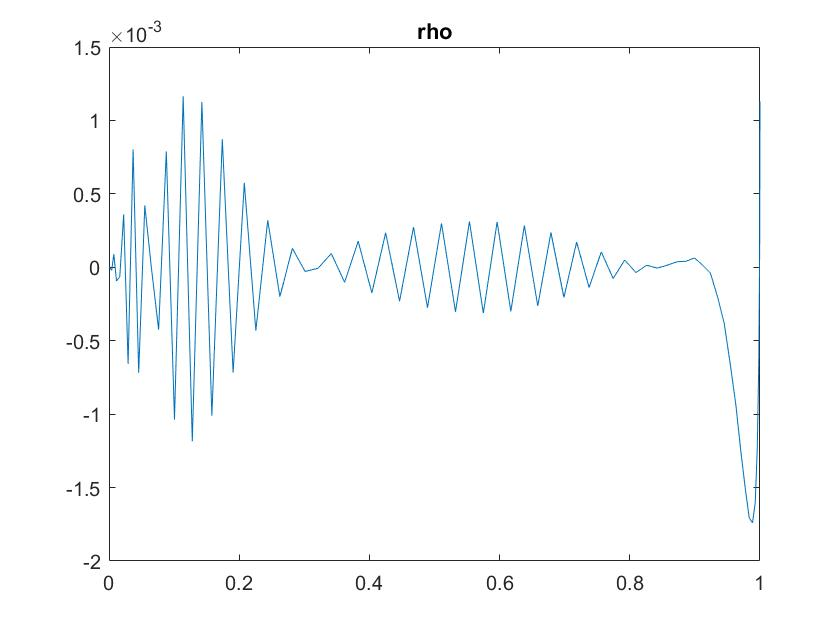
\includegraphics[scale=0.3]{Neumrho.jpg}
	\caption{Error in $p$ and $\rho$ at divergence point.}
\end{figure}
Using the exact $p$ as an initial guess does not help. We get a similar picture. \\
Then I tried to shift the exact solution of $p$ to match the one that we get by integrating the gradient equation (and adapt the exact solutions where necessary, i.e. $\hat \rho$). 
This is $p = \beta^{1/2} (e^T - e^t)(\cos(\pi y) +1)$.  Using this version of the exact solution did not improve the convergence either, so this doesn't seem to be caused by the issue with integration. This is backed up by the fact that the Dirichlet case has the same issues (see below).

\subsubsection*{Dirichlet Flow Control}
Tried perturbing the whole interval by $0.01f(t)$. This converges to a consistency of $0.00213573$ at Iteration 192. Both variables continued to converge more towards the exact solution: $\rho_{Err} = 0.00359323$ at Iteration 215 and $p_{Err} = 0.00213573$ at Iteration 244, then both diverge. Using a smaller $\lambda =0.01$, does not improve these results. The error in the solution looks irratic; see Figures 5,6,7.
\begin{figure}[h]
	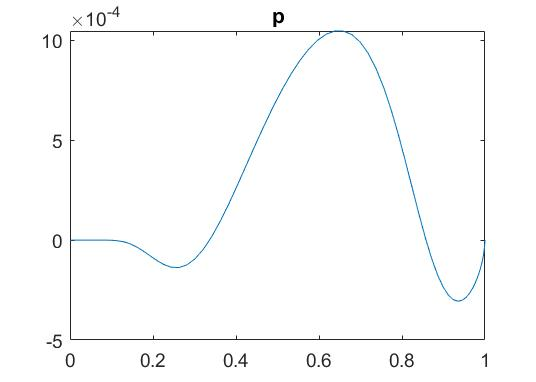
\includegraphics[scale=0.5]{pD3.jpg}
	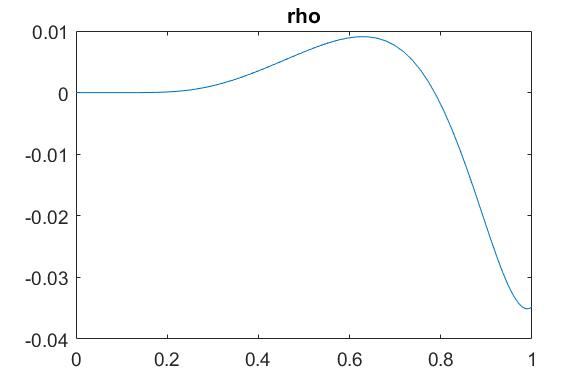
\includegraphics[scale=0.4]{rD3.jpg}
	\caption{Initial Error.}
\end{figure}
\begin{figure}[h]
	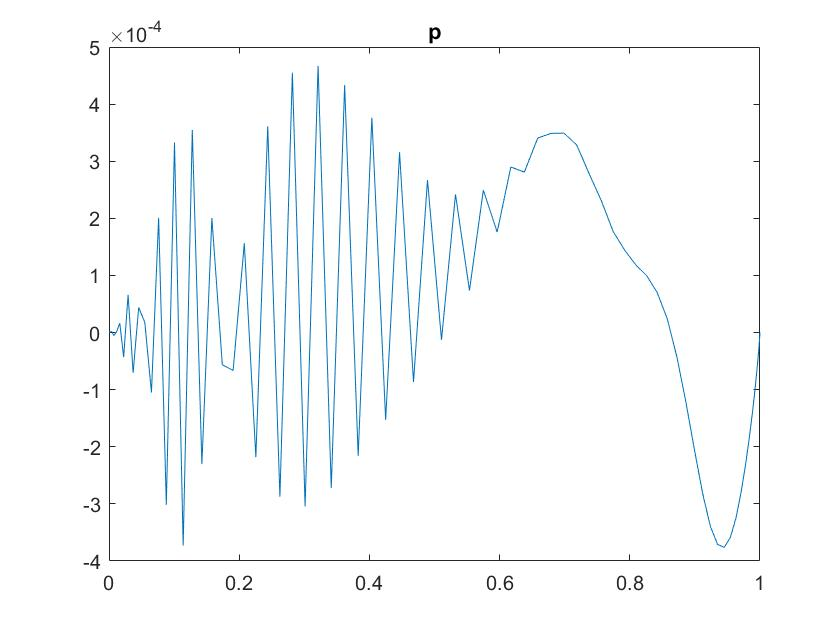
\includegraphics[scale=0.3]{pD2.jpg}
	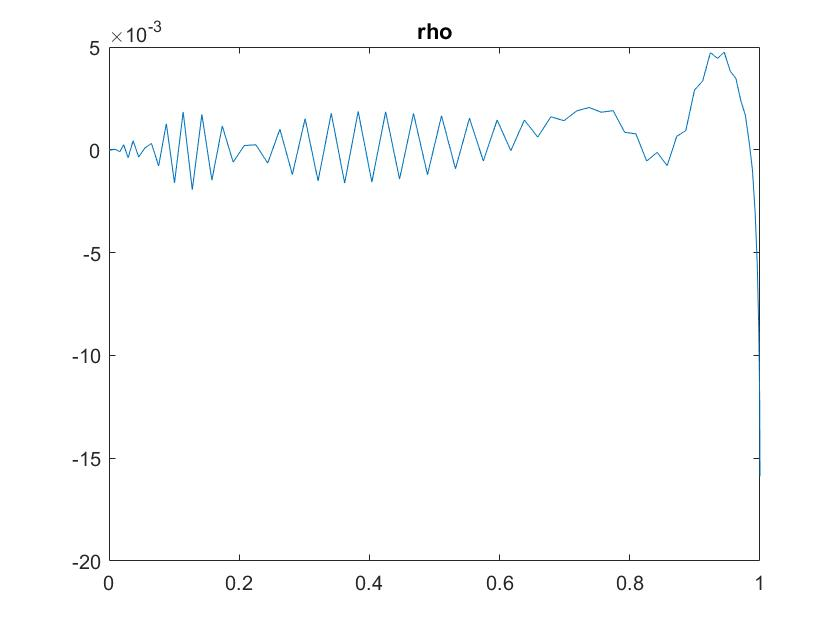
\includegraphics[scale=0.3]{rD2.jpg}
	\caption{Error at diverging point.}
\end{figure}
\begin{figure}[h]
	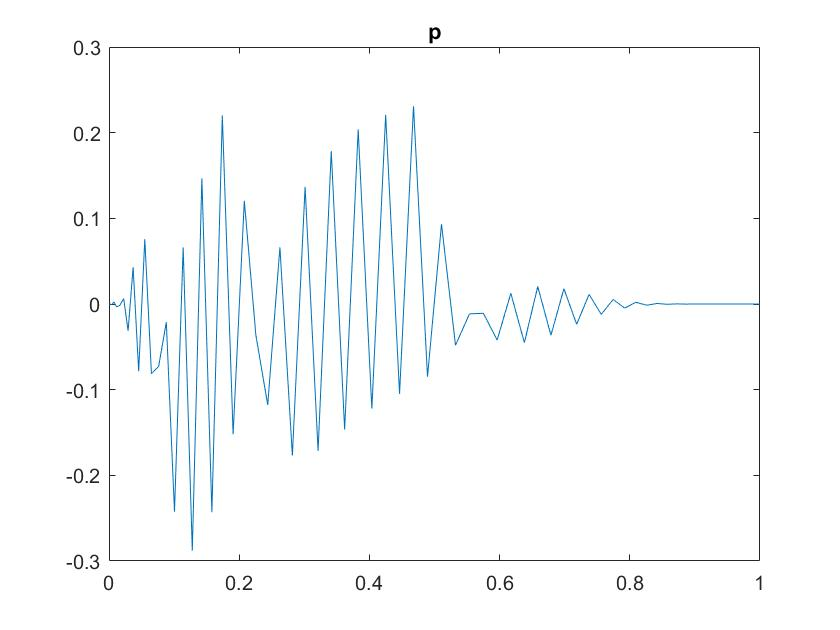
\includegraphics[scale=0.3]{pD1.jpg}
	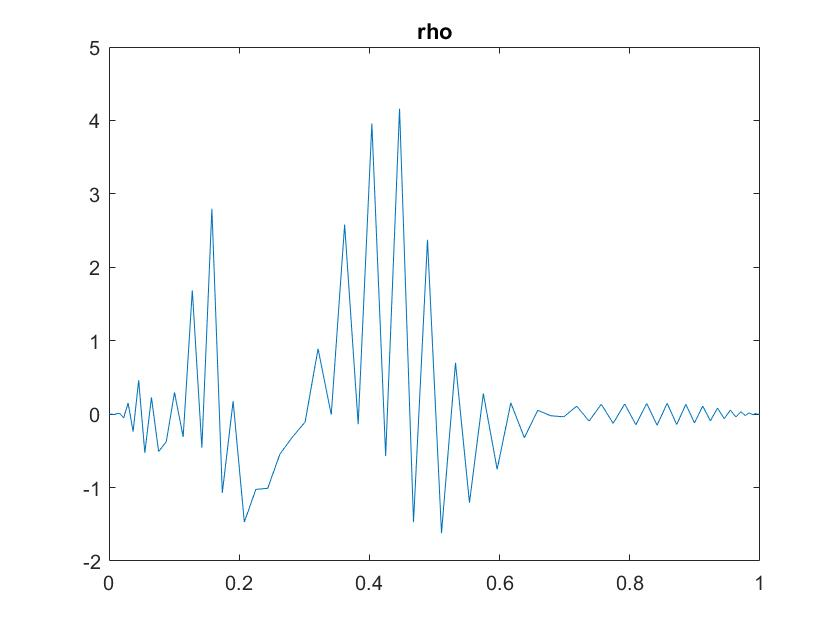
\includegraphics[scale=0.3]{rD1.jpg}
	\caption{Error past diverging point.}
\end{figure}


\subsubsection*{Mixed Boundary Conditions}
Since one of the issues were with the integration of the gradient equation to get $p$ and losing information there, I have tried to apply the mixed boundary conditions, using the following split:
\begin{align*}
0.99 (\frac{\partial \rho}{\partial n} + \rho w \cdot n ) + 0.01 \rho = 0\\
0.99 \frac{\partial p }{\partial n} + 0.01 p = 0.
\end{align*}
The perturbation $0.1ff(t)$ is applied, at $\beta = 10^{-1}$, ODE tolerances are here at $10^{-9}$. This converges, with exact errors $\rho_{err} = 0.00000149$ and $p_{Err} = 0.00001362$. 
The initial error in consistency is $0.08778247$. Now, changing $\beta = 10^{-3}$, results in an initial consistency error of $8.15134029$. With a $\lambda =0.1$, the errors fluctuate. Using $\lambda = 0.01$ it converges slowly. However, it reaches 5000 iterations at a consistency error of $0.00059962$. An adaptive approach resulted in fluctuations of errors again. 
Generally, I think it should be possible to get this to converge. It doesn't look as erratic as the solutions above.

\subsubsection*{Solving for the gradient of the adjoint equation}
The adjoint equation now solved for is:
\begin{align*}
\partial_t q = - \Delta q + \nabla (\hat \rho - \rho) - \nabla (w \cdot q)\\
q = 0 \qquad \text{on} \quad \partial \Omega,
\end{align*}
where $q = \nabla p$.
The gradient equation becomes:
\begin{align*}
w = - \frac{1}{\beta}q \rho.
\end{align*}
When perturbing this by $0.1 f(t)$, it doesn't converge. The consistency goes down to $0.00693900$ at Iteration 226, $\rho_{err} = 0.00362417$ at iteration 205 and $p_{err} = 0.00788789$ at Iteration 224. The errors are also here very erratic as seen above. 
Decreasing $\lambda =0.05$ does not help.\\
Choosing $0.01f(t)$ as perturbation also diverges before the consistency tolerance of $10^{-5}$ is reached.
\end{document}